\documentclass[nopalatino,nolot,nolof,color,11pt]{fithesis3/fithesis3}
\thesissetup{
  faculty=fi,
  type=mgr,
  author={Bc. Pavel Dedík},
  advisor={doc. Mgr. Radek Pelánek, Ph.D.},
  title={Modeling Students' Memory},
  keywords={memory, learning, knowledge, student modeling, performance factor analysis}}

\usepackage{lmodern}
\usepackage{amssymb}
\usepackage{graphicx}
\usepackage{enumitem}
\usepackage{algorithm}
\usepackage{mathtools}
\usepackage{booktabs,siunitx}
\usepackage[noend]{algpseudocode}

% To be removed when the thesis is finished.
\usepackage{lipsum}
\usepackage[marginpar]{todo}

\setlist[itemize]{leftmargin=10mm}

\begin{document}
  \chapter{Introduction}

Human memory has been studied by psychologists and neurologists for about 100 years~\cite{baddeley1997human}, it is the biological storage for the information acquired from past experience with the environment. There are many types of memory, all cooperating in the process of memorization. It may seem that memory is a single unitary system such as the heart, however, it is rather a collection of systems where for example one system is responsible for the encoding of new information while another helps with its storage over a long period of time.

The systems responsible for retention of information in the human brain are very closely related to \textit{learning} and \textit{forgetting}, both of which additionally depend to some extent on memory. That is true because our memory provides the means and structure to link new knowledge faster by association and inference. Hence, human memory is a \textit{complex system} and understanding the whole underlying process has been the interest of many researchers.

The exploration of human memory and learning has applications particularly in education, where our goal is to increase the amount of material students learn in one study session. Before the invention of computers and the growth of the Internet, the ways to test and evaluate new methods of educating students involved classrooms with usually only a limited number of participants. In the last 20 years, students and educational institutions started to use and develop new e-learning tools as a complimentary system for education. \textit{Adaptive educational systems} are systems that provide online environment for practicing different domains of educational content adaptively.

In adaptive educational systems, our effort is to create sufficiently accurate representation of students in order to make the system personalized, increase students' motivation and the speed of learning. A part of all adaptive systems are mathematical models which are constructed in order to model learning of individual students, adapt the system to students' abilities, behavior and knowledge of the subject. These models and their evaluation is very often based on \textit{machine learning} techniques and is also closely related to statistics. The ability to model the adaptive behavior also requires research connected to cognitive psychology. 

The goal of our thesis is to summarize the relevant research to modeling human memory and forgetting. Further, our goal is to design, evaluate and analyze models or extensions of the existing models used in adaptive educational systems. As we focus on the students of the online system \url{slepemapy.cz} (more chapter~\ref{outline-maps}), we are primarily concerned with students whose prior knowledge of the practiced material varies greatly.

\section{Outline Maps}
\label{outline-maps}

The analysis and evaluation of models is performed using the data from the on-line system \url{slepemapy.cz} for practicing geography~\cite{Papousek2014}. The practice of geography involves rehearsal of contextual information about a place on a map, i.e. the location, shape or neighbors of a country. The test of students' knowledge is done by presenting questions requiring the selection of correct associates between a name of a place and its position on an outline map (see Figure~\ref{fig:slepemapy}).

\begin{figure}[htbp]
  \centering
  \includegraphics[width=\textwidth]{img/slepemapy}
  \caption{The screenshot corresponds to a multiple-choice question (with 5 distractors) requiring the student to identify the name of the highlighted country on an outline map of Europe.}
  \label{fig:slepemapy}
\end{figure}

The system provides an educational environment for learning of all kinds of geography facts, including world countries, cities, rivers, lakes, mountains, islands, Czech regions and many others. The system is also adaptive, i.e. it examines knowledge and skills of individual students adaptively based on previous answers by the selection of optimal repeat frequency, the type of question and its difficulty.

\section{Outline of the Thesis}

The first chapter covers the background for of thesis, we summarize the most relevant aspects of human memory and forgetting related to our research, we also describe characteristics of adaptive educational systems as well as mathematical models used in student modeling. In the second chapter, we propose models and their modifications that focus on timing information, we also describe the numerous methods and metrics used for parameter estimation. In the last chapter, we evaluate and compare the proposed models on several data sets containing different types of places (countries, mountains, rivers, etc.), we analyze the stability of models' predictions and perform further analysis.

  \chapter{Background}

In this chapter we present an overview of the related research with the topic of our thesis. Firstly, we describe how the human brain can acquire new knowledge, the process of retention of information and the retrieval of information from memory. Secondly, we give an overview of the techniques suitable for educational systems with the focus on adaptive learning of facts.

\section{Student Modeling and Memory}

Throughout the last one hundred years, researchers have been trying to figure out the complex cognitive processes in the human brain, which are responsible for our ability to learn~\cite{RichardE.Mayer2010}. Understanding the process of learning can be very helpful in education and educational systems where we wish to improve the student's representation. This is useful if we want to adapt our system to the needs and knowledge of individual students practicing a particular domain (e.g. the knowledge of animals, Japanese vocabulary or geography). The construction of a quantitative representation, called a \textit{student model}, is known as \textit{student modeling}~\cite{Sison1998}.

The Greek philosopher and mathematician Plato compared human mind to an aviary in which each bird represented a memory~\cite{MichaelW.Eysenck2008}. Today, we have a much better intuition on the human biological storage -- the hardware responsible for the storage and organization of data in modern computers. This analogy of computer data storage is much better than the one Plato used and it seems to be very close and accurate depiction of the human memory.

So far, we haven't mentioned learning, which is very closely related to memory and to the topic of our thesis. Learning leads to the creation of memory. The study of learning and memory can be divided even further when we realize that we need some way to observe what the students know by experiments. This section is thus explained in three parts:

\begin{itemize}
  \item Learning
  \item Memory
  \item Performance
\end{itemize}

This distinction is not very important, however, it can help the reader better understand the underlying problem discussed in our thesis, the connection between computer science and psychology. In a book released by a professor of psychology at the University of California Richard~E.~Mayer, the science of learning is organized differently, that is into the following three components:

\begin{itemize}
  \item The science of learning
  \item The science of instruction
  \item The science of assessment
\end{itemize}

All of these components are to some extent related to our research. However, the science of learning is the most related since it concerns human memory and learning. The science of instruction is about the manipulation of the student's environment in order to foster learning, it's the scientific study of how to help people learn. In educational systems, this is usually done by incorporating \textit{instructional policies}, the strategies or a set of instructions that help students maintain engagement and increase the amount gained knowledge in one session. Instructional policies guide students during learning by e.g. the selection of appropriate questions or the number of options in multiple-choice tests. Lastly, the science of assessment seeks to determine what people know, which is important so that we are able to quantify the effectiveness of different instructional methods~\cite{RichardE.Mayer2010}.

\subsection{Learning}

\begin{figure}[htbp]
  \centering
  \includegraphics[width=\textwidth]{img/learning-forgetting-curves}
  \caption{Learning curve (left) and forgetting curve (right).}
  \label{fig:learning-forgetting-curves}
\end{figure}

Richard E. Mayer formulated learning as a change in what the student knows caused by the student's experience~\cite{RichardE.Mayer2010}. More specifically, learning is the process of encoding, modifying and reinforcing information~\cite{Lewis}. For example the encoding of the location of Portugal can be seen as learning the shape of the country, its neighbor Spain and the surrounding ocean.

A learning curve is the rate of the student's progress in gaining new skill or knowledge by experience in the environment (e.g. by participating in a discussion, reading a book or riding a bike). Generally, the speed of learning is proportional to the product of amount learned and amount to yet learn. This can be written mathematically:

\begin{equation} \label{learning-differential}
  \frac{dK}{dt} = a \cdot (K_{max} - K)
\end{equation}

The coefficient $a$ in the Equeation~\ref{learning-differential} represents the rate of learning. $K$ is the student's knowledge and $K_{max}$ the maximum knowledge possible. Several functions modeling the learning curve were proposed in the past, namely the power law, exponential and hyperbolic function. Most researchers nowadays believe that learning follows the power law~\cite{Klusasek2014}.

In order to model learning we need to be able to measure \textit{memory strength}, which is a measurement of the ability to retrieve an \textit{item} from memory. In our case an item is any information that can be learned. Memory strength can be measured indirectly by observing the following attributes of students when an item is practiced:

\begin{description}[leftmargin=0cm]
  \item[Probability of recall] Probability of the student recalling the practiced item, this can be measured as the fraction of the number of successful recollections and the number of all presentations.
  \item[Latency of recall] Latency of the student when retrieving the practiced item from memory. Latency of recall can be measured by observing the response times of students.
  \item[Savings in relearning] The number of required revisions of the practiced item in order to fully regain its knowledge~\cite{MichaelW.Eysenck2008}.
\end{description}

We can further distinguish the following levels of learning as measured by memory strength (portrayed on Figure~\ref{fig:knowledge-levels}):

\begin{figure}[htbp]
  \centering
  \includegraphics[width=\textwidth]{img/knowledge-levels}
  \caption{Different levels of learning.}
  \label{fig:knowledge-levels}
\end{figure}

\begin{description}[leftmargin=0cm]
  \item[Familiarity] The student has feeling they knew the item in the past but cannot remember anymore.
  \item[Recognition] The student recognized the item when presented multiple-choice options but couldn't remember otherwise.
  \item[Recall] The student is able to recall the item with some effort. Note that in cognitive science we distinguishe \textit{free recall} and \textit{cued recall}. Free recall is the ability to remember an item without any help (e.g. recalling the name of a country), in the case of cued recall, we are given an information which can help us remember (e.g. first letter of the country we are to remember).
  \item[Automaticity] The student recalls the item instantaneously when presented. Note that the level of automaticity can be measured by the latency of recall.
\end{description}

\subsection{Memory}

Memory is the biological storage that retains the information, e.g. the location of Portugal. The student's memory, however, decays with time. This memory decay is called \textit{forgetting} and similarly as learning it respects the power law.

Forgetting can be reduced by repetition. Repetition can be massed or spaced, in a massed presentation the item is revised in a short interval many times over. In contrast, a spaced presentation usually consists of revisions performed in a longer period of time with pauses between presentations. It is well known that a spaced presentation leads to a better memory strength~\cite{RichardE.Mayer2010}. This phenomenon is called the \textit{spacing effect}.

The next matter we haven't mentioned as of yet are the two kinds of long-term memory, that is the procedural (knowing how) and declarative (knowing what) memory. The procedural memory is the memory we aren't consciously aware and which makes humans capable of the acquisition of both the motor and cognitive skills. The declarative memory (sometimes referred as explicit memory) is the conscious knowledge such as the world's countries or the English vocabulary~\cite{MichaelW.Eysenck2008}.

\subsection{Performance}

The performance of students is the determination of what they know. Performance can be estimated from the speed and precision of recall, e.g. by a multiple-choice test, where the correctness of answers and response time is measured~\cite{Lewis}. Performance can be seen as an instrument that describes the student's knowledge, the understanding of which is important because it helps us guide the instructional policy.

\section{Relevant Student Models}
\label{relevant-models}

In this section we discuss the models relevant to our work. There are two main components that concern us. The first is the estimation of prior knowledge which can be helpful if we need better understanding of the student's acquired knowledge. The second is the estimation of the current knowledge which combines the knowledge the student already had and the knowledge they acquired. Estimation of current knowledge is significant for the better part of this thesis.

\subsection{Elo System}
\label{elo}

Elo system is a mathematical model suited for student modeling as recent research has shown. Elo rating system and its extension Glicko is otherwise a very popular approach in competitor-versus-competitor games such as chess~\cite{Vanek2014}. In our work we employ the model for the estimation of prior knowledge of students.

In the standard version of Elo system we have the student's skill $\theta_s$ and the difficulty of an item $b_i$. Equations~\ref{eq-elo-skill} and~\ref{eq-elo-difficulty} demonstrate an update of the student's skill and the item's difficulty after one answered question. The parameter $R$ is $0$ or $1$ depending on the correctness of the student's answer. The probability that a student with a given skill $\theta_s$ will answer correctly on the presented question of difficulty $b_i$ is estimated by a logistic function (see Equation~\ref{eq-elo-logistic}).

\begin{equation} \label{eq-elo-skill}
  \theta_s \gets \theta_s + K(R - P(R = 1|s,i))
\end{equation}

\begin{equation} \label{eq-elo-difficulty}
  b_i \gets b_i - K(R - P(R = 1|s,i))
\end{equation}

\begin{equation} \label{eq-elo-logistic}
  P(R = 1|s,i) = \frac{1}{1 + e^{-(\theta_s - b_i)}}
\end{equation}

The constant parameter $K$ affects the change in the estimates $\theta_s$ and $b_i$. Higher value means faster change after few questions, in contrast lower value makes the change slower. This is a problem since the number of answers varies throughout the time. It's been demonstrated that the use of an uncertainty function $\frac{a}{1 + bn}$, which considers the number of answers of students in the system, makes the predictions more stable and increases accuracy~\cite{Vanek2014}.

\subsection{Performance Factor Analysis}
\label{pfa}

Performance Factor Analysis (PFA) is a student modeling approach based on the Learning Factor Analysis (LFA). The standard PFA equation is formulated with the incorporation of knowledge components (KCs), which may include skills, concepts or facts~\cite{Pavlik2009}.

\begin{equation} \label{eq-pfa-standard}
  m(i,j \in KCs,s,f) = \sum_{j \in KCs} \beta_j + \gamma_j s_{i,j} + \delta_j f_{i,j} 
\end{equation}

\begin{equation} \label{eq-pfa-standard-p}
  P(m) = \frac{1}{1 + e^{-m}}
\end{equation}

In Equation~\ref{eq-pfa-standard}, where $m$ is a function of the student's knowledge, the parameter $\beta_j$ is the difficulty of the knowledge component $j$. The counts of current successes and failures of the student $i$ and the knowledge component $j$ are represented by the parameters $s_{i,j}$ and $f_{i,j}$, where $\gamma_j$ and $\delta_j$ define the weight of each success and failure.

The standard PFA model is defined in terms of knowledge components which is not always needed. The main disadvantage, however, is the inability to consider the order of answers. Another problem with the standard model is that it doesn't take into account the probability of guessing. Both these issues are solved in the following model:

\begin{equation} \label{eq-pfa-extended}
  m \gets \begin{cases}
            m + \gamma \cdot (1 - P(m)) & \text{\textbf{if }} \text{the answer was correct} \\
            m + \delta \cdot P(m) & \text{\textbf{otherwise}}
          \end{cases}
\end{equation}

\begin{equation} \label{eq-pfa-standard-p}
  P(m) = \frac{1}{n} + \left(1 - \frac{1}{n}\right)\frac{1}{1 + e^{-m}}
\end{equation}

The initial value of $m$ in Equation~\ref{eq-pfa-extended} can be estimated from the Elo model which was discussed in the section~\ref{elo}, i.e. $m = \theta_s - b_i$. The parameter $n$ in the Equation~\ref{eq-pfa-standard-p} matches the number of options in multiple-choice question. Note that the probability of guess is $\frac{1}{n}$ and the probability of slip is $1 - \frac{1}{n}$.

Another variation of the original PFA model was proposed by Yue Gong~\cite{Gong2011}. The idea of the model is based on the fact that we expect the student who answered in total of four presentations two times correctly in the last two presentations to perform better than the student who answered correctly in the first two presentations. The extended model introduces a decay factor $\xi$ that changes the behavior of the parameters $s_{i,j}$ and $f_{i,j}$ (see Equations~\ref{eq-pfa-gong-s},~\ref{eq-pfa-gong-f}).

\begin{equation} \label{eq-pfa-gong-s}
  s_{i,j} = \sum_{k=1}^{n-1} y_k \cdot \xi^{n-1-k}
\end{equation}

\begin{equation} \label{eq-pfa-gong-f}
  f_{i,j} = \sum_{k=1}^{n-1} |y_k - 1| \cdot \xi^{n-1-k}
\end{equation}

The parameter $y_k$ represents the correctness of the $k$-th question. 
The problem of this model is that it cannot be easily adjusted so that it includes the probability of guessing, particularly in cases where the practices were presented in the form of multiple-choice questions with varied number of options.

\todo{Some examples would be nice.}

\subsection{Models of Students' Memory}
\label{spacing-effect}

\todo{Nice plot showing what the hell this is all about.}

In the ACT-R model~\cite{Pavlik2003}, the memory strength $m$ of the student $s$ can be modeled by the Equation~\ref{eq-actr}.

\begin{equation} \label{eq-actr}
  m_n(t) = \ln{\sum_{i=1}^{n} t_{i}^{-d}}
\end{equation}

The parameter $t$ is a vector of seconds that passed since each of the $n$ repetitions were performed by the student $s$. The parameter $d$ represents memory decay (the speed of forgetting). Note that the equation is just a simplification of the reality and does not take into account many very important aspects of forgetting, e.g. the mentioned spacing effect.

Philip~I.~Pavlik and John~R.~Anderson~\cite{Pavlik2005} developed an extended version of the equation in which the decay is a function of the activation at the time the item was presented (see Equation~\ref{eq-pavlik-decay} and Equation~\ref{eq-pavlik-activation}).

\begin{equation} \label{eq-pavlik-decay}
  d_i = ce^{m_{i-1}} + a
\end{equation}
\begin{equation} \label{eq-pavlik-activation}
  m_n(t) = \ln{\sum_{i=1}^{n} t_{i}^{-d_i}}
\end{equation}

The parameters $c$ and $a$ affect the scale of the decay. Since $m_0 = -\infty$, the value of $d_i$ is always equal to $a$ for the first practice of the student. Additionally, when $c = 0$, the result of the equation is equivalent with the Equation~\ref{eq-actr}. Because the computation is recursive and a bit complex, we present the pseudo-code of the algorithm computing the memory activation function (see Algorithm~\ref{alg-memory-activation}).

\begin{algorithm}
  \caption{The function $\textsc{MemoryActivation}: \mathbb{N}^n \rightarrow \mathbb{R}^n$ takes the vector parameter $t$ in descending order, e.g. $[56800, 56400, 3600, 60, 0]$ (the last zero is the current practice). The result of the computation is a vector $m$ of student's memory strengths during each practice.}
  \label{alg-memory-activation}
  \begin{algorithmic}[1]
    \Function{MemoryActivation}{$t$}
      \State $n \gets size(t)$
      \State $m_0 \gets -\infty$
      \For{$i \gets 1$ \textbf{to} $n-1$}
        \State $s \gets 0$
        \For{$j \gets 1$ \textbf{to} $i$}
          \State $d_j \gets ce^{m_{j-1}} + a$
          \State $s \gets s + (t_j - t_i)^{-d_j}$
        \EndFor
        \State $m_i \gets \log(s)$
      \EndFor
      \State \Return $m$
    \EndFunction
  \end{algorithmic}
\end{algorithm}

\todo{Proof of correctness? Perhaps not necessary.}

Note that the time complexity of the function is $\mathcal{O}\left(\frac{n(n-1)}{2}\right)$.

  \chapter{Models Based on Timing Information}

The models presented in chapter~\ref{relevant-models} seem to work well in the context of adaptive systems. But could the performance be further improved by taking into account the timing information of students' answers (i.e. the response times or the breaks between practices)? As was discussed in chapter~\ref{spacing-effect}, the spacing effect is observable in environments where the students have no prior knowledge. We are interested primarily in domains where the prior knowledge varies widely between students.

\section{PFA and Timing}

In this chapter we discuss several models which aim at modeling students' memory with the usage of timing information of answers. There are several several issues to consider beforehand:

\begin{itemize}
  \item Students have different skills and thus the rate of retention loss varies.
  \item The difficulty of items varies, some items are forgotten faster and some slower.
  \item The prior knowledge of each student is different. If the student already has the practiced item in their long term memory, the process of forgetting is much slower.
\end{itemize}

\subsection{PFA with Forgetting}

One possibility how to incorporate timing information into the PFA model is by changing the memory activation in prediction. The times of previous attempts are passed to a \textit{time effect function} which may increase the probability of recall (see Equation~\ref{eq-pfa-standard-time-p}).

\begin{equation} \label{eq-pfa-standard-time-p}
  P(m) = \frac{1}{1 + e^{-(m + f(t))}}
\end{equation}

Since this is an extension of the standard PFA model, it is possible to integrate the estimation of prior knowledge as well as the probability of guessing into the model.

\subsection{PFA Gong with Forgetting}

Another way of dealing with timing between attempts is by changing the decay factor $\xi$ of the model presented in chapter~\ref{pfa}. The model takes into account the order of questions, yet doesn't consider timing between student's practices of an item. This problem can be resolved by replacing the parameter $\xi$ with a time effect function.

\begin{equation} \label{eq-pfa-gong-time-s}
  s_{i,j} = \sum_{k=1}^{n-1} y_k \cdot f(t_k)
\end{equation}

\begin{equation} \label{eq-pfa-gong-time-f}
  f_{i,j} = \sum_{k=1}^{n-1} |y_k - 1| \cdot f(t_k)
\end{equation}

Equations~\ref{eq-pfa-gong-time-s},~\ref{eq-pfa-gong-time-f} show the incorporation of the time effect function $f$ in the model. The parameter $t_k$ represents the number of seconds that passed between the $k$-th practice and the most recent one. The weight of successes and failures is thus dependent on the ages of the prior practices.

As was discussed in the chapter~\ref{pfa}, the problem arises with multiple-choice questions. Another difficulty is the choice of a time effect function that fits the data well. The function should theoretically represent the rate at witch the effect of learning decays with the passage of time.

  \chapter{Evaluation and Analysis}

In the first part of this section we briefly depict the nature of the data set used for evaluation of the models and discuss some specifics of the implementation. In the next part we present the results of our analysis.

\section{Data Set}

\todo{Add proper credit to the authors and developers of slepemapy.cz.}

For the analysis we used data from the online system for practicing geography\footnote{\url{http://www.slepemapy.cz}}~\cite{Papousek2014}. The data set contains more than 10~million answers from thousands of unique users~\cite{Papousek2015}. The data were filtered to contain only students with at least 50 answers and usually divided into 5 data sets, each containing at least 30 thousand answers. The answers of students who registered before the oldest question in the data set was answered were removed since it could temper with the results (considering we are interested primarily in models based on timing information).

\section{Toolchain}

The models were implemented in Python programming language. Experiments were performed in the Jupyter Notebook interactive environment\footnote{Jupyter Notebook is an open sourced web application for interactive computing, see~\url{https://jupyter.org/}}. Here is a list of the used libraries and modules:

\begin{itemize}
  \item SciPy, NumPy, Pandas
  \item Scikit-Learn
  \item Matplotlib
  \item NetworkX
\end{itemize}

\section{Response Time}

The response time of student to a question indicates how much well the item is learned. If the student answered quickly, almost automatically, it is very likely they either know the place very well or don't at all, depending on the correctness of their answer. On the other hand when the response is longer, the student is probably familiar with the item and might even recall the correct answer.

The Figure~\ref{fig-response-time} demonstrates the relationship between students' response time and the probability of recall. If the student's answer was suspiciously fast (response time is lower than 800 milliseconds), it usually means they guessed and don't know the correct answer. If the response time is between 1500 and 2000 milliseconds, it may indicate the student knows the place.

Note that some places are bigger on the map then other, i.e. a question requiring the student to choose Russia on the map has generally lower response time than a question requiring to choose Andorra.

\begin{figure}[htbp]
  \centering
  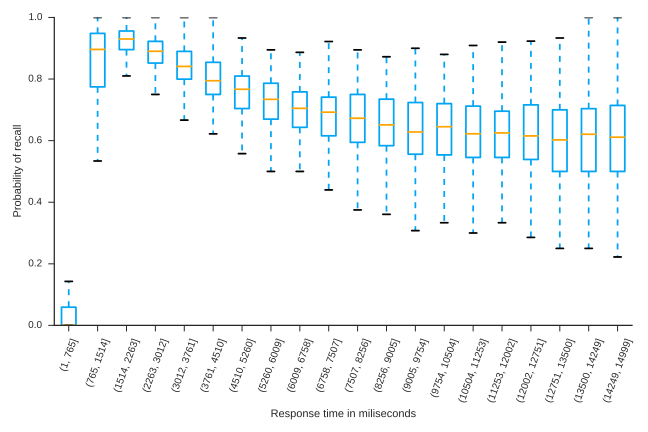
\includegraphics[width=\textwidth]{img/response-time}
  \caption{Relation between students' response time and probability of recall. Each box represents probabilities from all countries that belong in the relevant interval of response times.}
  \label{fig-response-time}
\end{figure}

\section{Calibration}

\section{Model Comparison}

\todo{The tables in this section aren't very readable, it should contain more information presented in a different way. Also it would be more interesting to adjust the parameters $\gamma$, $\delta$ for each data set.}

  \chapter{Conclusion}

In the first part of the thesis we summarized the key aspects of human memory, learning, and forgetting. We discussed applications and properties of adaptive educational systems, basics of student modeling and the most relevant models relevant in the context of our thesis, mainly the Elo model successfully used for estimation of prior knowledge of students and the Performance Factor Analysis (PFA) model used for the estimation of current knowledge the students acquired while interacting with the system. We also studied extensions of the PFA model and the models used in the ACT-R modeling system.

The primary objective of our thesis was to explore the family of PFA models and design their extensions while accounting for the key aspect of human memory---forgetting. We described several models based on previous extensions and introduced a \textit{time effect function} which penalizes the age of past attempts of an item. The evaluation of models was performed using the data from the adaptive system Outline Maps for practicing geography. Our evaluation showed that both models that focus on forgetting of students outperform their baseline models. We also analyzed students' response times for the possibility that it may indicate the level of student's knowledge, and the values of model's parameters depending on the domain of the used data set (the type of place, purpose of practice, etc.).

We suggested the usage of the extended PFA model with a staircase function in production, which is computationally very efficient and does not require periodic estimations of parameters. Other models do not perform so well especially in environments where the test of student's knowledge involves answer to a multiple-choice question.


  % To be removed when the thesis is finished.
  \todos
\end{document}
